\documentclass{standalone}
\usepackage{tikz}
\usetikzlibrary{patterns, positioning}

\begin{document}
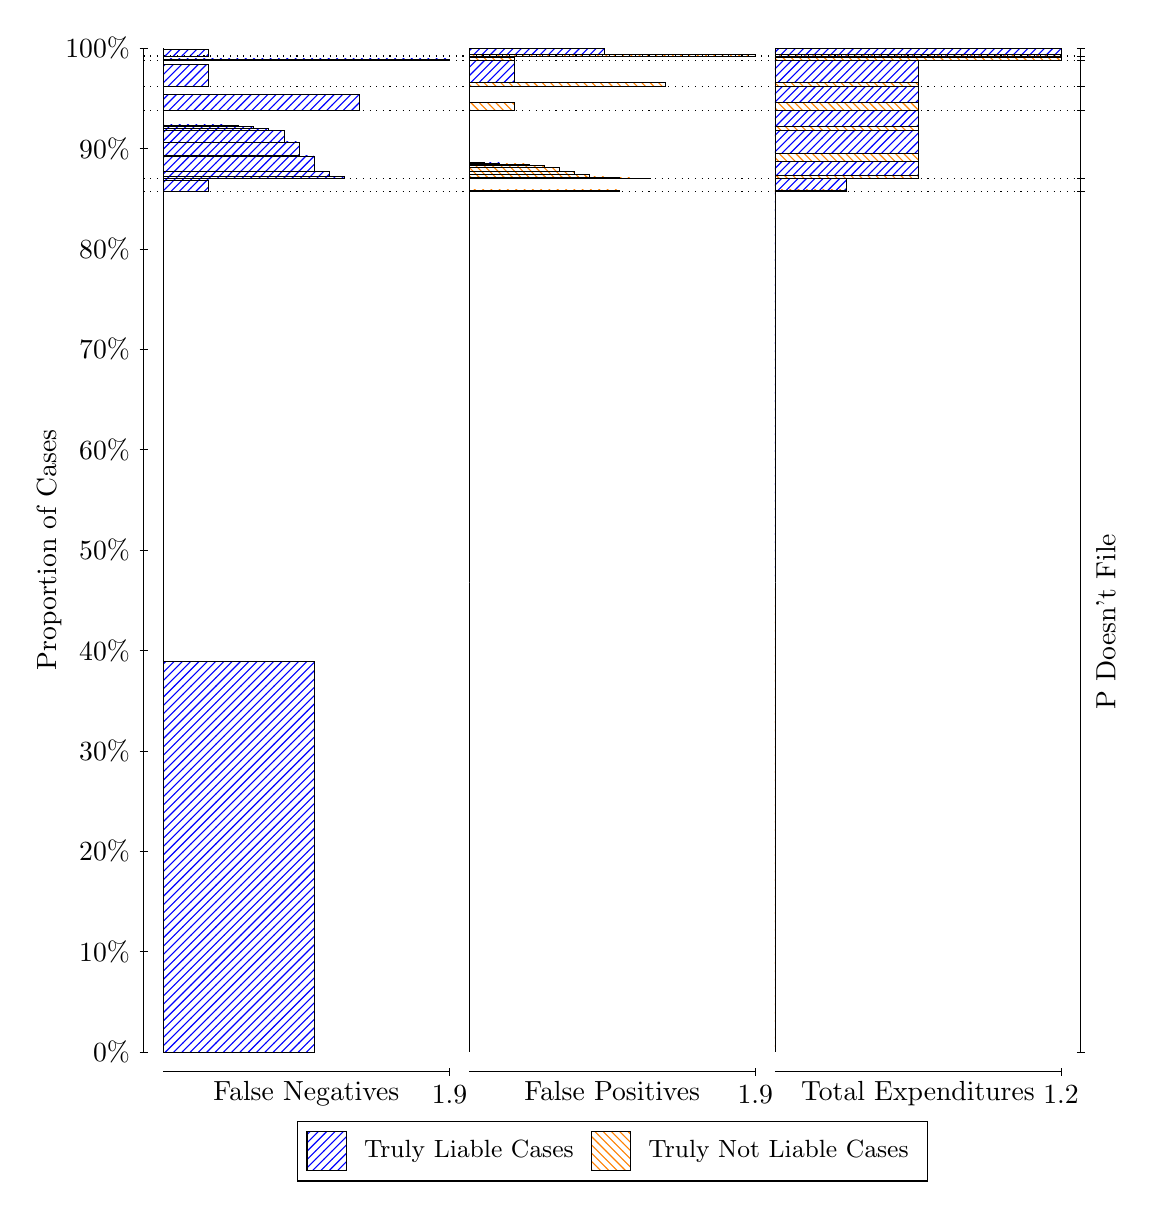
\begin{tikzpicture}
\draw[black, very thin] (1.5,1.75) -- (1.5,14.5);
\node[rotate=90, anchor=center] at (0.3, 8.125) {Proportion of Cases};
\draw[black, very thin] (1.45,1.75) -- (1.55,1.75);
\node[anchor=east] at (1.45, 1.75) {0\%};
\draw[black, very thin] (1.45,3.025) -- (1.55,3.025);
\node[anchor=east] at (1.45, 3.025) {10\%};
\draw[black, very thin] (1.45,4.3) -- (1.55,4.3);
\node[anchor=east] at (1.45, 4.3) {20\%};
\draw[black, very thin] (1.45,5.575) -- (1.55,5.575);
\node[anchor=east] at (1.45, 5.575) {30\%};
\draw[black, very thin] (1.45,6.85) -- (1.55,6.85);
\node[anchor=east] at (1.45, 6.85) {40\%};
\draw[black, very thin] (1.45,8.125) -- (1.55,8.125);
\node[anchor=east] at (1.45, 8.125) {50\%};
\draw[black, very thin] (1.45,9.4) -- (1.55,9.4);
\node[anchor=east] at (1.45, 9.4) {60\%};
\draw[black, very thin] (1.45,10.675) -- (1.55,10.675);
\node[anchor=east] at (1.45, 10.675) {70\%};
\draw[black, very thin] (1.45,11.95) -- (1.55,11.95);
\node[anchor=east] at (1.45, 11.95) {80\%};
\draw[black, very thin] (1.45,13.225) -- (1.55,13.225);
\node[anchor=east] at (1.45, 13.225) {90\%};
\draw[black, very thin] (1.45,14.5) -- (1.55,14.5);
\node[anchor=east] at (1.45, 14.5) {100\%};

\draw[black, very thin] (13.4,1.75) -- (13.4,14.5);
\draw[black, very thin] (13.35,1.75) -- (13.45,1.75);
\node[anchor=west] at (13.35, 1.75) {};
\draw[black, very thin] (13.35,12.677) -- (13.45,12.677);
\node[anchor=west] at (13.35, 12.677) {};
\draw[black, very thin] (13.35,12.844) -- (13.45,12.844);
\node[anchor=west] at (13.35, 12.844) {};
\draw[black, very thin] (13.35,13.71) -- (13.45,13.71);
\node[anchor=west] at (13.35, 13.71) {};
\draw[black, very thin] (13.35,14.008) -- (13.45,14.008);
\node[anchor=west] at (13.35, 14.008) {};
\draw[black, very thin] (13.35,14.343) -- (13.45,14.343);
\node[anchor=west] at (13.35, 14.343) {};
\draw[black, very thin] (13.35,14.399) -- (13.45,14.399);
\node[anchor=west] at (13.35, 14.399) {};
\draw[black, very thin] (13.35,14.5) -- (13.45,14.5);
\node[anchor=west] at (13.35, 14.5) {};

\draw[black, very thin, pattern color=blue, pattern=north east lines] (1.75,1.75) rectangle (3.6623,6.7152);
\draw[black, very thin, pattern color=orange, pattern=north west lines] (1.75,6.7152) rectangle (1.75,12.677);
\draw[black, very thin, pattern color=blue, pattern=north east lines] (1.75,12.677) rectangle (2.3237,12.825);
\draw[black, very thin, pattern color=orange, pattern=north west lines] (1.75,12.825) rectangle (1.75,12.844);
\draw[black, very thin, pattern color=blue, pattern=north east lines] (1.75,12.844) rectangle (4.0447,12.872);
\draw[black, very thin, pattern color=blue, pattern=north east lines] (1.75,12.872) rectangle (3.8535,12.931);
\draw[black, very thin, pattern color=blue, pattern=north east lines] (1.75,12.931) rectangle (3.6623,13.131);
\draw[black, very thin, pattern color=blue, pattern=north east lines] (1.75,13.131) rectangle (3.4711,13.14);
\draw[black, very thin, pattern color=blue, pattern=north east lines] (1.75,13.14) rectangle (3.4711,13.308);
\draw[black, very thin, pattern color=blue, pattern=north east lines] (1.75,13.308) rectangle (3.2798,13.454);
\draw[black, very thin, pattern color=blue, pattern=north east lines] (1.75,13.454) rectangle (3.0886,13.481);
\draw[black, very thin, pattern color=blue, pattern=north east lines] (1.75,13.481) rectangle (2.8974,13.503);
\draw[black, very thin, pattern color=blue, pattern=north east lines] (1.75,13.503) rectangle (2.7061,13.513);
\draw[black, very thin, pattern color=blue, pattern=north east lines] (1.75,13.513) rectangle (2.5149,13.525);
\draw[black, very thin, pattern color=orange, pattern=north west lines] (1.75,13.525) rectangle (1.75,13.71);
\draw[black, very thin, pattern color=blue, pattern=north east lines] (1.75,13.71) rectangle (4.236,13.907);
\draw[black, very thin, pattern color=orange, pattern=north west lines] (1.75,13.907) rectangle (1.75,14.008);
\draw[black, very thin, pattern color=blue, pattern=north east lines] (1.75,14.008) rectangle (2.3237,14.292);
\draw[black, very thin, pattern color=orange, pattern=north west lines] (1.75,14.292) rectangle (1.75,14.343);
\draw[black, very thin, pattern color=blue, pattern=north east lines] (1.75,14.343) rectangle (5.3833,14.363);
\draw[black, very thin, pattern color=orange, pattern=north west lines] (1.75,14.363) rectangle (1.75,14.399);
\draw[black, very thin, pattern color=blue, pattern=north east lines] (1.75,14.399) rectangle (2.3237,14.48);
\draw[black, very thin, pattern color=orange, pattern=north west lines] (1.75,14.48) rectangle (1.75,14.5);
\draw[black, very thin, pattern color=orange, pattern=north west lines] (5.6333,1.75) rectangle (5.6333,7.7118);
\draw[black, very thin, pattern color=blue, pattern=north east lines] (5.6333,7.7118) rectangle (5.6333,12.677);
\draw[black, very thin, pattern color=orange, pattern=north west lines] (5.6333,12.677) rectangle (7.5456,12.697);
\draw[black, very thin, pattern color=blue, pattern=north east lines] (5.6333,12.697) rectangle (5.6333,12.844);
\draw[black, very thin, pattern color=orange, pattern=north west lines] (5.6333,12.844) rectangle (7.9281,12.847);
\draw[black, very thin, pattern color=orange, pattern=north west lines] (5.6333,12.847) rectangle (7.7368,12.85);
\draw[black, very thin, pattern color=orange, pattern=north west lines] (5.6333,12.85) rectangle (7.5456,12.855);
\draw[black, very thin, pattern color=orange, pattern=north west lines] (5.6333,12.855) rectangle (7.3544,12.863);
\draw[black, very thin, pattern color=orange, pattern=north west lines] (5.6333,12.863) rectangle (7.1632,12.893);
\draw[black, very thin, pattern color=orange, pattern=north west lines] (5.6333,12.893) rectangle (6.9719,12.93);
\draw[black, very thin, pattern color=orange, pattern=north west lines] (5.6333,12.93) rectangle (6.7807,12.989);
\draw[black, very thin, pattern color=orange, pattern=north west lines] (5.6333,12.989) rectangle (6.5895,13.01);
\draw[black, very thin, pattern color=orange, pattern=north west lines] (5.6333,13.01) rectangle (6.3982,13.03);
\draw[black, very thin, pattern color=blue, pattern=north east lines] (5.6333,13.03) rectangle (6.0158,13.041);
\draw[black, very thin, pattern color=blue, pattern=north east lines] (5.6333,13.041) rectangle (5.8246,13.051);
\draw[black, very thin, pattern color=blue, pattern=north east lines] (5.6333,13.051) rectangle (5.6333,13.71);
\draw[black, very thin, pattern color=orange, pattern=north west lines] (5.6333,13.71) rectangle (6.207,13.811);
\draw[black, very thin, pattern color=blue, pattern=north east lines] (5.6333,13.811) rectangle (5.6333,14.008);
\draw[black, very thin, pattern color=orange, pattern=north west lines] (5.6333,14.008) rectangle (8.1193,14.06);
\draw[black, very thin, pattern color=blue, pattern=north east lines] (5.6333,14.06) rectangle (6.207,14.343);
\draw[black, very thin, pattern color=orange, pattern=north west lines] (5.6333,14.343) rectangle (6.207,14.379);
\draw[black, very thin, pattern color=blue, pattern=north east lines] (5.6333,14.379) rectangle (5.6333,14.399);
\draw[black, very thin, pattern color=orange, pattern=north west lines] (5.6333,14.399) rectangle (9.2667,14.419);
\draw[black, very thin, pattern color=blue, pattern=north east lines] (5.6333,14.419) rectangle (7.3544,14.5);
\draw[black, very thin, pattern color=orange, pattern=north west lines] (9.5167,1.75) rectangle (9.5167,7.7118);
\draw[black, very thin, pattern color=blue, pattern=north east lines] (9.5167,7.7118) rectangle (9.5167,12.677);
\draw[black, very thin, pattern color=orange, pattern=north west lines] (9.5167,12.677) rectangle (10.425,12.697);
\draw[black, very thin, pattern color=blue, pattern=north east lines] (9.5167,12.697) rectangle (10.425,12.844);
\draw[black, very thin, pattern color=orange, pattern=north west lines] (9.5167,12.844) rectangle (11.333,12.882);
\draw[black, very thin, pattern color=blue, pattern=north east lines] (9.5167,12.882) rectangle (11.333,13.06);
\draw[black, very thin, pattern color=orange, pattern=north west lines] (9.5167,13.06) rectangle (11.333,13.162);
\draw[black, very thin, pattern color=blue, pattern=north east lines] (9.5167,13.162) rectangle (11.333,13.458);
\draw[black, very thin, pattern color=orange, pattern=north west lines] (9.5167,13.458) rectangle (11.333,13.503);
\draw[black, very thin, pattern color=blue, pattern=north east lines] (9.5167,13.503) rectangle (11.333,13.71);
\draw[black, very thin, pattern color=orange, pattern=north west lines] (9.5167,13.71) rectangle (11.333,13.811);
\draw[black, very thin, pattern color=blue, pattern=north east lines] (9.5167,13.811) rectangle (11.333,14.008);
\draw[black, very thin, pattern color=orange, pattern=north west lines] (9.5167,14.008) rectangle (11.333,14.06);
\draw[black, very thin, pattern color=blue, pattern=north east lines] (9.5167,14.06) rectangle (11.333,14.343);
\draw[black, very thin, pattern color=orange, pattern=north west lines] (9.5167,14.343) rectangle (13.15,14.379);
\draw[black, very thin, pattern color=blue, pattern=north east lines] (9.5167,14.379) rectangle (13.15,14.399);
\draw[black, very thin, pattern color=orange, pattern=north west lines] (9.5167,14.399) rectangle (13.15,14.419);
\draw[black, very thin, pattern color=blue, pattern=north east lines] (9.5167,14.419) rectangle (13.15,14.5);
\draw[black, dotted] (1.5,12.677) -- (13.4,12.677);
\draw[black, dotted] (1.5,12.844) -- (13.4,12.844);
\draw[black, dotted] (1.5,13.71) -- (13.4,13.71);
\draw[black, dotted] (1.5,14.008) -- (13.4,14.008);
\draw[black, dotted] (1.5,14.343) -- (13.4,14.343);
\draw[black, dotted] (1.5,14.399) -- (13.4,14.399);
\draw[black, very thin] (1.75,1.5) -- (5.3833,1.5);
\node[anchor=north] at (3.5667, 1.5) {False Negatives};
\draw[black, very thin] (5.3833,1.45) -- (5.3833,1.55);
\node[anchor=north] at (5.3833, 1.45) {1.9};

\draw[black, very thin] (5.6333,1.5) -- (9.2667,1.5);
\node[anchor=north] at (7.45, 1.5) {False Positives};
\draw[black, very thin] (9.2667,1.45) -- (9.2667,1.55);
\node[anchor=north] at (9.2667, 1.45) {1.9};

\draw[black, very thin] (9.5167,1.5) -- (13.15,1.5);
\node[anchor=north] at (11.333, 1.5) {Total Expenditures};
\draw[black, very thin] (13.15,1.45) -- (13.15,1.55);
\node[anchor=north] at (13.15, 1.45) {1.2};

\node[black, centered, rotate=90] at (13.72, 7.2135) {P Doesn't File};







\draw (7.449999999999999,1.5) node[draw=none] (baseCoordinate) {};
\begin{scope}[align=center]
        \matrix[scale=0.5, draw=black, below=0.5cm of baseCoordinate, nodes={draw}, column sep=0.1cm]{
            \node[rectangle, draw, minimum width=0.5cm, minimum height=0.5cm, pattern=north east lines, pattern color=blue] {}; &
            \node[draw=none, font=\small] (B) {Truly Liable Cases}; &
            \node[rectangle, draw, minimum width=0.5cm, minimum height=0.5cm, pattern=north west lines, pattern color=orange] {}; &
            \node[draw=none, font=\small] (B) {Truly Not Liable Cases}; \\
            };
\end{scope}

\end{tikzpicture}
\end{document}